% Format A4, podstawowa czcionka 12pt, wyjustowany
\documentclass[12pt,a4paper,twoside]{article}

% zażółć gęślą jaźń
\usepackage[utf8]{inputenc}
\usepackage[polish]{babel}
\usepackage{polski}

% Marginesy: 3cm, *2cm
\usepackage[left=3cm,right=2cm,top=2cm,bottom=2cm]{geometry}

% Times New Roman
\usepackage[T1]{fontenc}
\usepackage{mathptmx}

% wyrownanie numeru strony do lewej
\usepackage{fancyhdr}
\fancyhf{}
\renewcommand{\headrulewidth}{0pt}
\lfoot{\thepage}

% znormalizowanie nagłówków sekcji do 12pt
\usepackage{sectsty}
\sectionfont{\fontsize{12}{15}\selectfont}
\subsectionfont{\fontsize{12}{15}\selectfont}
\subsubsectionfont{\fontsize{12}{15}\selectfont}

% wciecie akapitow 10mm
\setlength{\parindent}{1cm}

% interlinia 1.5
\usepackage{setspace}
\onehalfspacing

% Dodawanie rysunków
\usepackage{graphicx}

% podpisy 10pt

\usepackage[font=footnotesize,labelfont=it]{caption}

\usepackage[polish]{babel}
\usepackage{polski}
\usepackage{fullpage}
\usepackage[utf8]{inputenc}
\usepackage{amsmath}
\usepackage{graphicx}
\usepackage[colorinlistoftodos]{todonotes}
\usepackage{listings}
\usepackage{caption}
\DeclareCaptionFont{white}{\color{white}}
\DeclareCaptionFormat{listing}{\colorbox{gray}{\parbox{\textwidth}{#1#2#3}}}
\captionsetup[lstlisting]{format=listing,labelfont=white,textfont=white}

\usepackage{color}

\definecolor{mygreen}{rgb}{0,0.6,0}
\definecolor{mygray}{rgb}{0.5,0.5,0.5}
\definecolor{mymauve}{rgb}{0.58,0,0.82}

\lstset{ %
  backgroundcolor=\color{white},   % choose the background color; you must add \usepackage{color} or \usepackage{xcolor}
  basicstyle=\footnotesize,        % the size of the fonts that are used for the code
  breakatwhitespace=false,         % sets if automatic breaks should only happen at whitespace
  breaklines=true,                 % sets automatic line breaking
  captionpos=t,                    % sets the caption-position to bottom
  commentstyle=\color{mygreen},    % comment style
  deletekeywords={...},            % if you want to delete keywords from the given language
  escapeinside={\%*}{*)},          % if you want to add LaTeX within your code
  extendedchars=true,              % lets you use non-ASCII characters; for 8-bits encodings only, does not work with UTF-8
  keepspaces=true,                 % keeps spaces in text, useful for keeping indentation of code (possibly needs columns=flexible)
  keywordstyle=\color{blue},       % keyword style
  language=Java,                 % the language of the code
  otherkeywords={*,...},            % if you want to add more keywords to the set
  numbers=left,                    % where to put the line-numbers; possible values are (none, left, right)
  numbersep=5pt,                   % how far the line-numbers are from the code
  numberstyle=\tiny\color{mygray}, % the style that is used for the line-numbers
  showspaces=false,                % show spaces everywhere adding particular underscores; it overrides 'showstringspaces'
  showstringspaces=false,          % underline spaces within strings only
  showtabs=false,                  % show tabs within strings adding particular underscores
  stepnumber=2,                    % the step between two line-numbers. If it's 1, each line will be numbered
  stringstyle=\color{mymauve},     % string literal style
  tabsize=2,                       % sets default tabsize to 2 spaces
}

\title{Badania wrażliwości proponowanej platformy obliczeniowej na rozmiar lokalnej grupy roboczej dla urządzeń OpenCL}

\author{Paweł J. Wal}

\date{\today}

\begin{document}

\maketitle

\section{CEL ZADANIA}

Celem zadania było sprawdzenie wrażliwości proponowanej platformy obliczeniowej na rozmiar lokalnej grupy roboczej na jednym z wykorzystywanych urządzeń obliczeniowych. Wykonanie tej pracy jest istotne z punktu widzenia projektu magisterskiego pod tytułem ,,Implementacja solwera frontalnego zrównoleglonego w wielowęzłowym heterogenicznym środowisku sprzętowym''.

\section{WYKORZYSTANE URZĄDZENIE}

Ze względu na czasową niedostępność urządzeń NVidia Tesla na węźle obliczeniowym Jack, badania zostały przeprowadzone przy użyciu procesora Intel Xeon X5650, działającego z prędkością 2.67GHz. Fakt wykorzystania tego urządzenia może mieć istotny wpływ na wyniki przeprowadzonych badań ze względu na fundamentalnie różną strukturę urządzeń typu CPU oraz GPU.

Procesor Intel Xeon X5650 może na raz przetwarzać do 12 wątków \cite{intel}. W rzeczywistości nie jest to idealna sytuacja, gdyż w procesorze tym zastosowano technologię Hyper-Threading. W istocie 12 wątków przetwarza jedynie 6 rdzeni; zwiększenie ilości wątków osiągnięte jest przy pomocy przetwarzania z przeplotem. Nie powoduje to jednak znaczącego wzrostu wydajności w aplikacjach takich jak wykorzystywany solwer.

W kontraście do procesora Intel Xeon X5650, GPU NVidia Tesla M2090 ma 512 dyskretnych rdzeni \cite{nvidia}. Ze względu na tą różnicę, urządzenia może charakteryzować inna optymalna wielkość grupy roboczej.

\section{METODA PRZEPROWADZENIA BADAŃ}

Jako obiecujące zostało wytypowanych pięć wartości badanego parametru: 1024, 512, 256, 128 i 16 wątków na grupę roboczą. Początkowo wartość 16 nie miała być uwzględniona, została jednak dodana do zestawu badanych wartości ze względu na specyfikę badanego urządzenia - konkretnie ze względu na niską ilość fizycznych rdzeni.

Każdy test wykonywany był w tych samych warunkach, a mianowicie: 

\begin{itemize}
\item klaster w stanie spoczynku (brak dodatkowych zadań),
\item macierz o rozmiarach 10000 x 10000 zmiennych,
\item rozmiar globalnej przestrzeni wątków równy 1024.
\end{itemize}

\begin{table}
\begin{center}
\begin{tabular}{|r|l|}
\hline
Rozmiar grupy roboczej & Czas [s] \\
\hline
1024 & 149,6132 \\ 
512	& 149,59215 \\
256	& 148,0225 \\
128	& 146,8443 \\ 
16	& 116,0606 \\
\hline
\end{tabular}
\end{center}
\caption{Średni czas obliczeń w zależności od badanego parametru}
\label{tab:time}
\end{table}

Dla każdej z wybranych wartości zostało przeprowadzonych 10 testów. Z uzyskanych czasów następnie wyliczone zostały wartości średnie, przedstawione w tablicy \ref{tab:time}. Graficznie wyniki przedstawia wykres przedstawiony na rysunku \ref{fig:lws}.

\begin{figure}
  \centering
    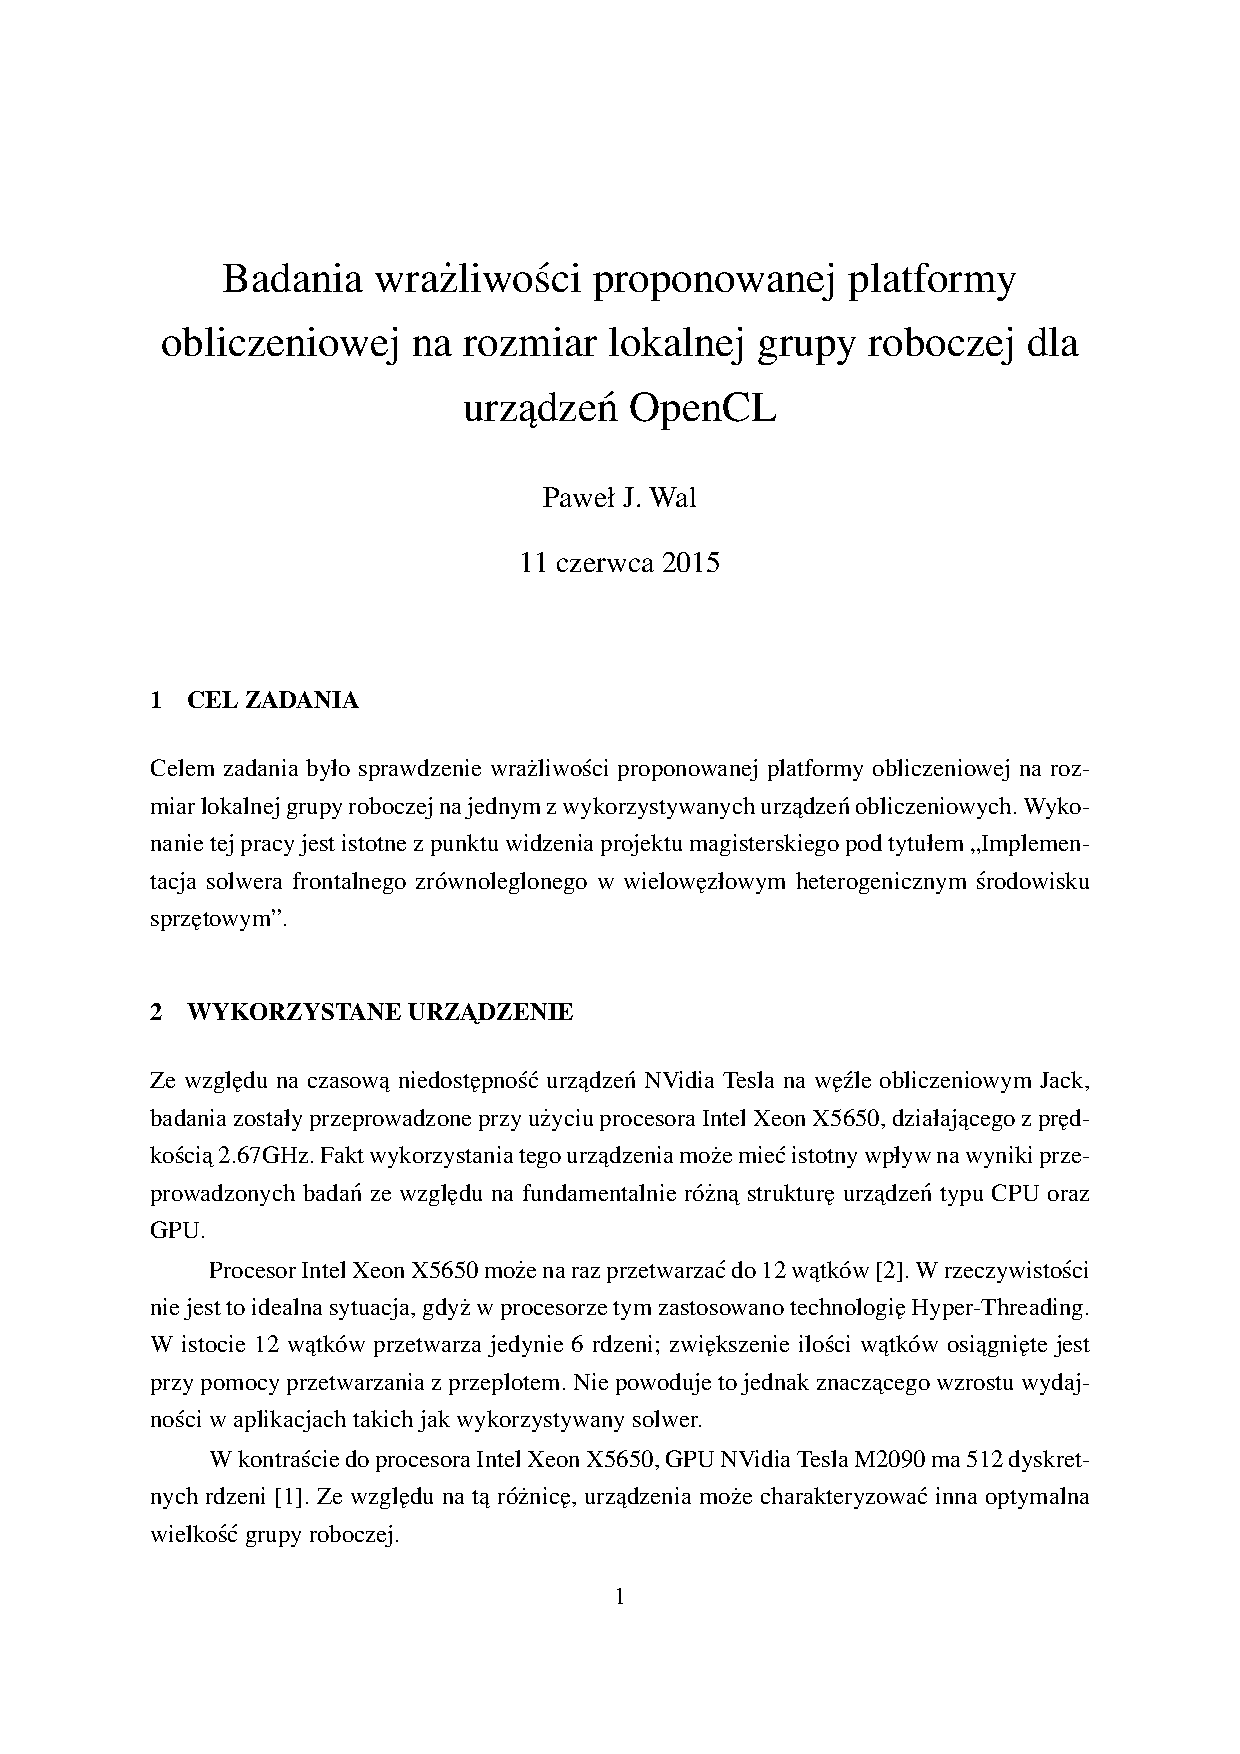
\includegraphics[width=0.9\textwidth]{lws}
  \caption{Graficzne przedstawienie średniego czasu obliczeń}
  \label{fig:lws}
\end{figure}

\section{WNIOSKI}

Jak łatwo zauważyć, dla najmniejszego badanego rozmiaru grupy roboczej czas obliczeń był najkrótszy. W dodatku jest to różnica niebagatelna - o niemal 30 sekund. W obliczeniach trwających około dwóch-dwóch i pół minuty jest to różnica dość znaczna.

Lepsze funkcjonowanie procesora dla mniejszych wartości badanego parametru jest zbieżne z przedstawionymi informacjami o jego konstrukcji. Większe rozmiary grup roboczych (zazwyczaj odpowiadające ilości fizycznych rdzeni bądź połowie tej wartości) są odpowiedniejsze dla urządzeń GPU, gdzie dyskretnych mikrordzeni jest znacznie więcej.

Niestety, w czasie pisania niniejszego projektu GPU Tesla M2090 nie były dostępne ze względu na problemy w konfiguracji węzła obliczeniowego. W ramach projektu magisterskiego konieczne będzie przeprowadzenie dodatkowych badań na tych urządzeniach i porównanie wyników.

Uzyskane podczas przedstawionych w niniejszym sprawozdaniu badań wyniki będą bardzo przydane w dalszym rozwoju projektu magisterskiego pod tytułem ,,Implementacja solwera frontalnego zrównoleglonego w wielowęzłowym heterogenicznym środowisku sprzętowym''. Wyniki te zwracają uwagę na problem doboru optymalnej wielkości grupy roboczej dla poszczególnych klas urządzeń. Być może do zestawu benchmarków uruchamianego podczas pierwszego uruchomienia klienta dołączyć należy również serię testów ustalających najlepszy rozmiar grupy roboczej dla danego urządzenia.

\section{BIBLIOGRAFIA}

\begingroup
\renewcommand{\section}[2]{}%
\begin{thebibliography}{99}

\bibitem{nvidia} Tesla M2090 Dual-Slot Computing Processor Module. Board Specification. \textit{NVIDIA}. 2012

\bibitem{intel} Intel Xeon Processor X5650 [online]. \textit{Intel ARK}. [dostęp: 2015-06-10], Dostępny w Internecie: <http://ark.intel.com/products/47922/Intel-Xeon-Processor-X5650-12M-Cache-2\_66-GHz-6\_40-GTs-Intel-QPI>

\end{thebibliography}
\endgroup

\end{document}